% ОБЯЗАТЕЛЬНО ИМЕННО ТАКОЙ documentclass!
% (Основной кегль = 14pt, поэтому необходим extsizes)
% Формат, разумеется, А4
% article потому что стандарт не подразумевает разделов
% Глава = section, Параграф = subsection
% (понятия "глава" и "параграф" из документа, описывающего диплом)
\documentclass[a4paper,article,14pt]{extarticle}

% Подключаем главный пакет со всем необходимым
\usepackage{spbudiploma_tempora}

% Пакеты по желанию (самые распространенные)
% Хитрые мат. символы
\usepackage{euscript}
% Таблицы
\usepackage{longtable}
\usepackage{makecell}
% Картинки (можно встявлять даже pdf)
\usepackage[pdftex]{graphicx}
% Удобные дифференциалы
\usepackage{physics}
% Матрицы и таблицы
\usepackage{amsmath}
\usepackage{multirow}

\usepackage{amsthm,amssymb, amsmath}
\usepackage{textcomp}
\usepackage{yfonts}


\begin{document}

% Титульник в файле titlepage.tex
% --------------------- Титульник ВКР СПбГУ -----------------------------
% Автор: Тоскин Николай, itonik@me.com
% Если заметили ошибку, напишите на email
% Если хотите добавить изменение самостоятельно:
% https://github.com/itonik/spbu_diploma/
% Использованы материалы:
% habr.com/ru/post/144648/
% cpsconf.ru
% Документы ниже могут уже быть неактуальны, тем не менее за годы ничего
% нового не появилось
% Текст:
% http://edu.spbu.ru/images/data/normativ_acts/local/20181030_10432_1.pdf
% Титульный лист:
% http://edu.spbu.ru/images/data/normativ_acts/local/20180703_6616_1.pdf
% -----------------------------------------------------------------------

% Титульный лист диплома СПбГУ
% Временное удаление foot на titlepage
\newgeometry{left=30mm, top=20mm, right=15mm, bottom=20mm, nohead, nofoot}
\begin{titlepage}
\begin{center}

\textbf{Санкт--Петербургский}
\textbf{государственный университет}

\vspace{35mm}

\textbf{\textit{\large Жестоканов Евгений Вячеславович}} \\[8mm]
% Название
\textbf{\large Выпускная квалификационная работа}\\[3mm]
\textbf{\textit{\large Структурный подход в мононеявных методах Рунге — Кутты}}

\vspace{20mm}
Уровень образования: бакалавриат\\
Направление 01.03.02 «Прикладная математика и информатика»\\
Основная образовательная программа СВ.5005.2015
«Прикладная математика, фундаментальная информатика и программирование»\\
Профиль «Исследование и проектирование систем управления\\ и обработки сигналов»\\[25mm]


% Научный руководитель, рецензент
\begin{flushright}
\begin{minipage}[t]{0.65\textwidth}
{Научный руководитель:} \\
кандидат физ.-мат. наук, доцент кафедры информационных систем Еремин~Алексей Сергеевич 

\vspace{10mm}

{Рецензент:} \\
профессор, кафедра компьютерных технологий \\и систем, д.ф. - м.н. Веремей~Евгений Игоревич
\end{minipage}
\end{flushright}

\vfill 

{Санкт-Петербург}
\par{\the\year{} г.}
\end{center}
\end{titlepage}
% Возвращаем настройки geometry обратно (то, что объявлено в преамбуле)
\restoregeometry
% Добавляем 1 к счетчику страниц ПОСЛЕ titlepage, чтобы исключить 
% влияние titlepage environment
\addtocounter{page}{1}


% Содержание
\tableofcontents
\pagebreak

\specialsection{Введение}
В процессе развития классических методов численного решения обыкновенных дифференциальных уравнений (ОДУ), таких как методы Рунге — Кутты (РК), экстраполяции и Адамса, которые изначально были разработаны для ручного расчёта, наблюдается постоянное расширение спектра решаемых задач, обусловленное технологическим прогрессом в области компьютерных вычислений.

С ростом мощности вычислительных машин появляются новые возможности для решения более сложных задач. Вместе с этим возникают и новые проблемы, связанные с приближением и устойчивостью более эффективных и надёжных алгоритмов численного интегрирования систем обыкновенных дифференциальных уравнений (СОДУ).

Отсутствие однородности в реальных задачах, когда встречаются задачи, которые не являются исключительно жёсткими или нежёсткими, а представляют собой их сочетание, стало важным стимулом для улучшения и развития численных методов решения как жёстких, так и нежёстких задач.

Рассматриваемая далее система вида (\ref{eq:base_system}) возникает при описании задач небесной механики, оптимального управления, физики высоких энергий \cite{OlemskoyBook2009}.
\pagebreak

\specialsection{Постановка задачи}
Методы решения структурно разделенных систем обыкновенных дифференциальных уравнений класса \textswab{A}(2) хорошо себя зарекомендовали с точки зрения критерия "вычислительные затраты/точность". Они позволяют получить требуемый порядок за меньшее число этапов, чем классический метод РК.

С другой стороны для жестких задач используются неявные методы РК, однако требуют наибольшего времени вычисления и ресурсов. Поскольку при их использовании возникает необходимость в решении векторной нелинейной системы.

Также для жестких задач используют моно-неявные методы РК, так как они хорошо себя показывают в решении жестких задач с вычислительной точки зрения \cite{mirk}.

В связи с двумя вышеперечисленными пунктами возникла мысль об объединении этих двух методов для анализа поведения полученного метода на жестких и нежестких задачах. Поскольку он должен вычисляться быстрее чем неявный РК, поскольку ему не нужно решать нелинейную систему, а только несколько нелинейных уравнений. А также должен неплохо себя показывать на жестких задачах.

В рамках данной работы планируется построить метод 4-го порядка: вывести условия порядка, предложить схему, а также рассмотреть вопрос об устойчивости данного метода. 
\pagebreak

\specialsection{Обзор литературы}
Для написания данной работы были изучены и использованы научная и учебно-методическая литература, статьи студентов факультета прикладной математики - процессов управления.

Значительное количество исследований, посвящённых численным методам решения систем обыкновенных дифференциальных уравнений (ОДУ), сосредоточено на подходах, основанных на разбиении системы на две (реже — более) подсистемы, к каждой из которых применяется свой численный метод. При этом, несмотря на различие методов, они остаются взаимосвязанными. Одними из первых стратегий такого рода стали разделения на линейные и нелинейные, а также на жёсткие и нежёсткие компоненты (см., например,\cite{Hofer1976}). В дальнейшем подобные подходы применялись для выделения быстрых и медленных процессов в сложных системах\cite{ShomeEtAl2004, SanduGuenther2016}, при решении уравнений в частных производных~\cite{KetchesonEtAl2016}, а также при разработке симплектических методов~\cite{KalogiratouEtAl2011}.

Среди методов такого рода особое внимание заслуживает подход, предложенный И.В.Олемским. Основу разделения в этом случае составляет структура зависимости правых частей системы ОДУ от её неизвестных функций. Было установлено, что во многих ситуациях возможно построение явных методов типа Рунге—Кутты, позволяющих достичь заданного порядка точности с меньшим числом вычислений правых частей по сравнению с классическими методами Рунге—Кутты, применяемыми без предварительного разделения. В частности, Олемскому удалось распространить идею, лежащую в основе методов Рунге—Кутты—Нюстрёма\cite{tree}, на системы, разбитые на две части с перекрёстной зависимостью. В ряде его работ были предложены методы третьего порядка с двумя этапами, четвёртого — с тремя\cite{Olemskoy2003}, и пятого порядка — с четырьмя этапами~\cite{Olemskoy2002}.

Моно-неявные методы РК(MIRK) активно изучаются в научной литературе множеством авторов на протяжении более тридцати лет. Изначально один из подклассов этих методов был предложен для решения задачи Коши в работе \cite{Cash1975}. Полный класс методов MIRK был представлен для задач с начальным значением в работах \cite{Bokhoven1980} и \cite{Cash1982}. Обзор существующих методов содержится в \cite{Muir1987}.

Для задач начального значения по ОДУ применение MIRK-схем оказывается по вычислительным затратам сопоставимым с лучшими реализациями более общего класса неявных методов РК (IRK). Что касается задач с граничными условиями (BVP), MIRK-методы анализировались в \cite{Cash1980}, \cite{Cash1982}, \cite{Enright1986} и \cite{Gupta1985}. При решении таких задач они могут быть реализованы столь же эффективно, как и явные методы Рунге-Кутты \cite{Enright1986}.

Методы MIRK применялись при разработке программного пакета HAGRON, ориентированного на численное решение граничных задач с использованием отложенных поправок \cite{Cash1991}. Более того, недавно MIRK-схемы были внедрены в другой программный комплекс, использующий непрерывные расширения этих методов для контроля дефектов при численном решении BVP-задач \cite{Muir1993}.

Основная часть указанных публикаций была посвящена разработке конкретных MIRK-методов и их эффективной реализации. Кроме того, в работах \cite{Bokhoven1980} и \cite{Gupta1985} проводился анализ условий порядка для MIRK-методов и их связи с классическими условиями Бутчера, характерными для стандартных IRK-схем. Более полный анализ подклассов с малым числом этапов и максимальным порядком s-этапного метода дан в \cite{mirk}. 

\pagebreak

\section{Существующие методы}
\subsection{Система}
Все дальнейшие рассуждения, кроме \ref{subsecMIRK} будем вести о следующей системе:
\begin{equation}
\begin{cases}
         \dv{y_1}{x} &= f_1(x,y_2), \\
         \dv{y_2}{x} &= f_2(x,y_1),
\end{cases}
\label{eq:base_system}
\end{equation}
\begin{equation}
    y_{s}(X_{0}) = y_{s0}, \quad s = 1,2, \quad x \in [X_{0},X_{1}] \subset R.
\end{equation}
\subsection{Структурный метод}
По \cite{OlemskoyBook2009} схема рассчета для структурного метода РК описывается:
\begin{equation}
    y_{s,i+1} = y_{s,i} + h \sum_{l=1}^{m_{s}} b_{sl} k_{sl} \quad s = 1, 2,
\end{equation}
\begin{equation}
\begin{aligned}
    k_{1l} &= 
\begin{cases}
    f_{1}(x + c_{11} h, y_{2i}), \quad l = 1, \\
    f_{1}(x + c_{1l} h, y_{2i} + h \sum_{n=1}^{l-1} a_{1ln} k_{2n}), \quad l = 2, \dotsc, m_{1},
\end{cases}
    \\k_{2l} &= 
    f_{2}(x + c_{2l} h, y_{1i} + h \sum_{n=1}^{l-1} a_{2ln} k_{1n}), \quad c_{21} \not= 0, l = 1, \dotsc, m_{2},
\end{aligned}
\end{equation}
\subsection{Мононеявный метод}\label{subsecMIRK}
По \cite{mirk} схема рассчета для моно-неявного метода РК описывается:
\begin{equation}
    y_{i+1} = y_{i} + h \sum_{l=1}^{s} b_{l} k_{l},
\end{equation}
\begin{equation}
    k_{l} = 
    f(x + c_{l} h, (1 - v_{l}) y_{1i} + v_{l} y_{1,i+1} + h \sum_{n=1}^{s} x_{ln} k_{n}), \quad l = 1, \dotsc, s.
\end{equation}
\pagebreak

\section{Предложенный метод}
\subsection{Схема}
\begin{equation}
    y_{s,i+1} = y_{s,i} + h \sum_{l=1}^{m_{s}} b_{sl} k_{sl} \quad s = 1, 2,
    \label{eq:method}
\end{equation}
\begin{equation}
\begin{aligned}
    k_{1l} &= 
\begin{cases}
    f_{1}(x + c_{11} h, (1 - v_{11}) y_{2i} + v_{11} y_{2,i+1}), \quad l = 1 \\,
    f_{1}(x + c_{1l} h, (1 - v_{11}) y_{2i} + v_{11} y_{2,i+1} + h \sum_{n=1}^{l-1} x_{1ln} k_{2n}), \quad l = 2, \dotsc, m_{1},
\end{cases}
    \\k_{2l} &= 
    f_{2}(x + c_{2l} h, (1 - v_{2l}) y_{1i} + v_{2l} y_{1,i+1} + h \sum_{n=1}^{l-1} x_{2ln} k_{1n}), \quad c_{21} \not= 0, l = 1, \dotsc, m_{2},
\end{aligned}
\label{eq:method_k}
\end{equation}
\begin{equation}
    m_{s_{1}} = 3 \quad m_{s_{2}} = 2.
\end{equation}
Коэффициенты в общем виде можно объединить в матрицы и векторы
\begin{equation}
C_{1} =
\begin{pmatrix}
    c_{1,1} & 0 & 0 \\
    0 & c_{1,2} & 0 \\
    0 & 0 & c_{1,3}
\end{pmatrix},
\end{equation}
\begin{equation}
C_{2} =
\begin{pmatrix}
    c_{2,1} & 0 \\
    0 & c_{2,2}
\end{pmatrix},
\end{equation}
\begin{equation}
X_{1} = 
\begin{pmatrix}
    0 & 0 \\
    x_{1,2,2,1} & 0 \\
    x_{1,3,2,1} & x_{1,3,2,2}
\end{pmatrix},
\end{equation}
\begin{equation}
X_{2} = 
\begin{pmatrix}
    x_{2,1,1,1} & 0 & 0\\
    x_{2,2,1,1} & x_{2,2,1,2} & 0 
\end{pmatrix},
\end{equation}
\begin{equation}
    v_{1} = \left[
    v_{1,2,1}, v_{1,2,2}, v_{1,2,3}
    \right],
\end{equation}
\begin{equation}
    v_{2} = \left[
    v_{2,1,1}, v_{2,1,2}
    \right],
\end{equation}
\begin{equation}
    b_{1} = \left[
    b_{1,1}, b_{1,2}, b_{1,3}
    \right],
\end{equation}
\begin{equation}
    b_{2} = \left[
    b_{2,1}, b_{2,2}
    \right].
\end{equation}
Введем вспомогательные матрицы и вектора для удобства записи условий порядка.
\begin{equation}
I_{i} = \underbrace{\left[
    1, \dotsc, 1
    \right]}_{i},
\end{equation}
\begin{equation}
A_{1} = 
\begin{pmatrix}
    v_{1,2,1} b_{2,1} & v_{1,2,1} b_{2,2} \\
    v_{1,2,2} b_{2,1} + x_{1,2,2,1} & v_{1,2,2} b_{2,2} \\
    v_{1,2,3} b_{2,1} + x_{1,3,2,1} & v_{1,2,3} b_{2,2} + x_{1,3,2,2}
\end{pmatrix},
\end{equation}
\begin{equation}
A_{2} = 
\begin{pmatrix}
    v_{2,1,1} b_{1,1} + x_{2,1,1,1} & v_{2,1,1} b_{1,2} & v_{2,1,1} b_{1,3}\\
    v_{2,1,2} b_{1,1} + x_{2,2,1,1} & v_{2,1,2} b_{1,2} + x_{2,2,1,2} & v_{2,1,2} b_{1,3}
\end{pmatrix}.
\end{equation}

\subsection{Условия порядка}\label{order_conditions}
Условия порядка для предложенного метода 4-го порядка. Полученны как удовлетворенные условия на соответствующие деревья из \cite{tree}.
Далее для s = 1, 2
\begin{equation}
U_{1} = I_{3}, \quad U_{2} = I_{2},
\end{equation}
\begin{equation}
A_{s} U_{s} - C_{s} U_{s},
\end{equation}
\begin{equation}
B_{s} U_{s} = 1,
\end{equation}
\begin{equation}
B_{s} C_{s}^{i} U_{s} = \frac{1}{i+1}, \quad i = 1, 2, 3,
\end{equation}
\begin{equation}
B_{s} A_{s} C_{s}^{i} U_{s} = \frac{1}{6i}, \quad i = 1, 2,
\end{equation}
\begin{equation}
B_{s} C_{s} A_{s} C_{s} U_{s} = \frac{1}{8},
\end{equation}
\begin{equation}
B_{s} A_{s} A_{s} C_{s} U_{s} = \frac{1}{24}.
\end{equation}

\subsection{Удовлетворенные условия}\label{conditions}
Далее будут приведены коэффициенты, удовлетворяющие условиям из \ref{order_conditions}. При их вычислении два раза были выбраны корни для квадратных уравнений, после чего получилась система с одним параметром $x_{132}$. Параметр был выбран равный 0.

\begin{equation}
    c_{1} = \left[
    1, \frac{2}{3} + \frac{\sqrt{2}}{6}, \frac{\sqrt{2}}{6}
    \right],
\end{equation}
\begin{equation}
    c_{2} = \left[
    \frac{1}{2} - \frac{\sqrt{3}}{6}, \frac{2}{3} + \frac{\sqrt{2}}{6}, \frac{\sqrt{2}}{6}
    \right],
\end{equation}
\begin{equation}
    v_{1} = \left[
    1, \frac{2}{3} + \frac{\sqrt{2}}{6} - \frac{\sqrt{3}}{6} + \frac{\sqrt{6}}{18}, \frac{-\sqrt{6}}{6} + \frac{\sqrt{2}}{6} + \frac{\sqrt{3}}{18}
    \right],
\end{equation}
\begin{equation}
    v_{2} = \left[
    \frac{2}{3} - \frac{\sqrt{3}}{6}, \frac{4}{3} - \frac{\sqrt{2}}{3} + \frac{\sqrt{3}}{6}
    \right],
\end{equation}
\begin{equation}
    b_{1} = \left[
    \frac{-1}{17} - \frac{3\sqrt{2}}{17}, \frac{3}{4}, \frac{21}{68} + \frac{3\sqrt{2}}{17}
    \right],
\end{equation}
\begin{equation}
    b_{2} = \left[
    \frac{1}{2}, \frac{1}{2}
    \right],
\end{equation}
\begin{equation}
X1 = 
\begin{pmatrix}
    0, 0\\
    \frac{-\sqrt{6}}{18} + \frac{\sqrt{3}}{6}, 0\\
    \frac{\sqrt{6}}{6} - \frac{\sqrt{3}}{18}, 0
\end{pmatrix},
\end{equation}
\begin{equation}
X2 = 
\begin{pmatrix}
    \frac{-1}{6}, 0, 0\\
    \frac{1}{6} + \frac{\sqrt{2}}{3}, -1, 0
\end{pmatrix}.
\end{equation}

Удовлетворенные условия порядка в общем виде можно посмотреть в репозитории \cite{code}.
\pagebreak

\section{Численные эксперименты}\label{numeric}
Проведем эксперименты для установления порядка метода. Вышепредложенный метод реализован на языке Python с использованием бибилотек NumPy и SciPy. Программный код реализации доступен в \cite{code}. Рассмотрим две задачи. \newline
Задача 1.
\begin{equation}
\begin{aligned}
    y_{1}' &= -y_{2} + e^{-x}, \\
    y_{2}' &= y_{1} + e^{-x}, \\
    x_{0} &= 0, y_{1}(0) = y_{2}(0) = 1, x_{end} = 1,
\end{aligned}
\end{equation}
Аналитическое решение выглядит следующим образом
\begin{equation}
\begin{aligned}
    y_{1} &= 2 \cos(x) - \sin(x) - e^{-x}, \\
    y_{2} &= 2 \sin(x) + \cos(x).
\end{aligned}
\end{equation}
Решаем задачу с постоянным шагом h. Порядок будем определять по форумле (\ref{eq:order}).
\begin{equation}
p = \log_{2}(\frac{E_{h}}{E_{\frac{h}{2}}})
\label{eq:order}
\end{equation}
Далее приведена таблица с глобальной прогрешностью $E_{h}$ в зависимости от шага h. 
\begin{center}
\begin{tabular}{ |c|c|c|c|c| } 
\hline
h & 0.1& 0.05 & 0.025 & 0.0125 \\ 
\hline
$E_{h}$ & $1.46050\cdot10^{-6}$ & $8.32381\cdot10^{-8}$ & $5.20788\cdot10^{-9}$ & $3.29724\cdot10^{-10}$ \\ 
\hline
\end{tabular}
\end{center}
Рассчитаем \ref{eq:order} для каждых двух соседних столбцов.
\begin{equation}
\log_{2}(\frac{E_{0.1}}{E_{0.05}}) = 4.13307, \quad \log_{2}(\frac{E_{0.05}}{E_{0.025}}) = 3.99848 , \quad \log_{2}(\frac{E_{0.025}}{E_{0.0125}}) = 3.98137
\end{equation}
Из чего можем сделать вывод, что порядок для этой задачи соблюдается. \newline
Задача 2.
\begin{equation}
\begin{aligned}
    y_{1}' &= -y_{2} + e^{-20x}, \\
    y_{2}' &= y_{1} + e^{-20x}, \\
    x_{0} &= 0, y_{1}(0) = y_{2}(0) = 1, x_{end} = 1,
\end{aligned}
\end{equation}
Аналитическое решение выглядит следующим образом
\begin{equation}
\begin{aligned}
    y_{1} &= \frac{422}{401} \cos(x) - \frac{420}{401} \sin(x) - \frac{21}{401 e^{20x}}, \\
    y_{2} &= \frac{420}{401} \cos(x) + \frac{422}{401} \sin(x) - \frac{19}{401 e^{20x}}.
\end{aligned}
\end{equation}
Далее приведена таблица с глобальной прогрешностью $E_{h}$ в зависимости от шага h.
\begin{center}
\begin{tabular}{ |c|c|c|c|c| } 
\hline
h & 0.1& 0.05 & 0.025 & 0.0125 \\ 
$E_{h}$ & $2.97881\cdot10^{-4}$ & $2.10493\cdot10^{-5}$ & $1.37051\cdot10^{-6}$ & $8.69485\cdot10^{-8}$ \\ 
\hline
\end{tabular}
\end{center}
Рассчитаем \ref{eq:order} для каждых двух соседних столбцов.
\begin{equation}
\log_{2}(\frac{E_{0.1}}{E_{0.05}}) = 3.82289 , \quad \log_{2}(\frac{E_{0.05}}{E_{0.025}}) = 3.94099 , \quad \log_{2}(\frac{E_{0.025}}{E_{0.0125}}) = 3.97841
\end{equation}
Из чего можем сделать вывод, что порядок для этой задачи соблюдается c небольшой погрешность для самого большого шага.
\pagebreak

\section{Устойчивость метода}
\subsection{Функция устойчивости в общем виде}
\begin{equation}
\begin{cases}
    y_{1}'(x) = \lambda y_{2}(x), \\
    y_{2}'(x) = \lambda y_{1}(x).
\end{cases}
\label{eq:test_system}
\end{equation}

Для получения функции устойчивости для предложенного метода рассмотрим результат применения одного шага метода (\ref{eq:method}) к системе (\ref{eq:test_system}). Можем рассматривать уравнение с одинаковыми собственными числами, поскольку систему с любыми двумя собственными числами можно свести к такому виду \cite{stability}.

\begin{equation}
\begin{aligned}
    y_{11} = y_{10} + z b_1^T Y_{12}, \\
    y_{21} = y_{20} + z b_2^T Y_{21},
\end{aligned}    
\label{eq:one_step}
\end{equation}
$Y_{12}$ и $Y_{21}$ представляют собой вектора вида.
\begin{equation}
\begin{aligned}
Y_{12} = \left[
Y_{121}, \dotsc, Y_{12m_{1}}
\right], \\
Y_{21} = \left[
Y_{211}, \dotsc, Y_{21m_{2}}
\right],
\end{aligned}
\end{equation}
Выражаем $Y_{12i}$ и $Y_{21i}$ согласно (\ref{eq:method_k}), учитывая особенности системы (\ref{eq:test_system}).
\begin{equation}
\begin{aligned}
    Y_{12i} = (1 - v_{1i}) y_{20} + v_{1i} y_{21} + \sum_{j=1}^{i-1} x_{12ij} f_{2} (Y_{21j}),\\
    Y_{21i} = (1 - v_{2i}) y_{10} + v_{2i} y_{11} + \sum_{j=1}^{i} x_{21ij} f_{1} (Y_{12j}),
\end{aligned}
\label{eq:Y_i}
\end{equation}
Запишем уравнения (\ref{eq:Y_i}) в векторном виде.
\begin{equation}
\begin{aligned}
    Y_{21} = (I_{s2} - v_{2}) y_{10} + v_{2} y_{11} + z X_{21} Y_{12}, \\
    Y_{12} = (I_{s1} - v_{1}) y_{20} + v_{1} y_{21} + z X_{12} Y_{21},
\end{aligned}
\end{equation}
Далее запишем матричное уравнение.
\begin{equation}
    \begin{pmatrix} Y_{12}\\ Y_{21} \end{pmatrix}
    = \begin{pmatrix}
        E & -z X_{12} \\
        -z X_{21} & E
    \end{pmatrix}^{-1}
    \begin{pmatrix}
        (I_{s1} - v_{1}) y_{20} + v_{1} y_{21} \\
        (I_{s2} - v_{2}) y_{10} + v_{2} y_{11}
    \end{pmatrix},
\label{eq:Y_matrix}
\end{equation}
Подставим (\ref{eq:Y_matrix}) в (\ref{eq:one_step})
\begin{equation}
    \begin{pmatrix} y_{11}\\ y_{21} \end{pmatrix}
    = 
    \begin{pmatrix} y_{10}\\ y_{20} \end{pmatrix}
    + z
    \begin{pmatrix}
         b_{1}^{T} & 0 \dotsc 0 \\
         0 \dotsc 0 & b_{2}^{T}
    \end{pmatrix}
    \begin{pmatrix}
        E & -z X_{12} \\
        -z X_{21} & E
    \end{pmatrix}^{-1}
    \begin{pmatrix}
        (I_{s1} - v_{1}) y_{20} + v_{1} y_{21} \\
        (I_{s2} - v_{2}) y_{10} + v_{2} y_{11}
    \end{pmatrix},
\end{equation}
Введем обозначение и через него выразим уравнение выше.
\begin{equation}
\begin{pmatrix}
         b_{1}^{T} & 0 \dotsc 0 \\
         0 \dotsc 0 & b_{2}^{T}
    \end{pmatrix}
    \begin{pmatrix}
        E & -z X_{12} \\
        -z X_{21} & E
    \end{pmatrix}^{-1}
=:
\begin{pmatrix}
    d_{11} & d_{12} \\
    d_{21} & d_{22}
\end{pmatrix},
\end{equation}
\begin{equation}
    \begin{pmatrix} y_{11}\\ y_{21} \end{pmatrix}
    = 
    \begin{pmatrix} y_{10}\\ y_{20} \end{pmatrix}
    + z
    \begin{pmatrix}
    d_{11} & d_{12} \\
    d_{21} & d_{22}
    \end{pmatrix}
    \left[
    \begin{pmatrix}
        (I_{s1} - v_{1}) y_{20} \\
        (I_{s2} - v_{2}) y_{10} 
    \end{pmatrix}
    +
    \begin{pmatrix}
        v_{1} y_{21} \\
        v_{2} y_{11} 
    \end{pmatrix}
    \right],
\end{equation}
Раскроем полседнюю скобку и приведем подобные слагаемые.
\begin{equation}
\begin{pmatrix}
    1 - z d_{12} v_{2} & -z d_{11} v_{1} \\
    -z d_{22} v_{2} & 1 - z d_{21} v_{1}
\end{pmatrix}
\begin{pmatrix} y_{11}\\ y_{21} \end{pmatrix}
=
\begin{pmatrix}
    1 + z d_{12} (I_{s2} - v_{2}) & z d_{11} (I_{s1} - v_{1}) \\
    z d_{22} (I_{s2} - v_{2}) & 1 + z d_{21} (I_{s1} - v_{1})
\end{pmatrix}
\begin{pmatrix} y_{10}\\ y_{20} \end{pmatrix},
\end{equation}
Выразим уравнение выше через (\ref{eq:P}) и (\ref{eq:stability_general})
\begin{equation}
P(z, w_{1}, w_{2}) = 
\begin{pmatrix}
    1 + z d_{12} w_{2} & z d_{11} w_{1} \\
    z d_{22} w_{2} & 1 + z d_{21} w_{1}
\end{pmatrix},
\label{eq:P}
\end{equation}
\begin{equation}
    R(z) = P^{-1}(z , -v_{1}, -v_{2}) P(z, I_{s1} - v_{1}, I_{s2} - v_{2}),
    \label{eq:stability_general}
\end{equation}
Окончательно получаем
\begin{equation}
\begin{pmatrix} y_{11}\\ y_{21} \end{pmatrix}
    = R(z)
\begin{pmatrix} y_{10}\\ y_{20} \end{pmatrix}.
\end{equation}

\subsection{Функция устойчивости для предложенного метода}

Подставим в (\ref{eq:stability_general}) коэффициенты из \ref{conditions}.
\begin{equation}
\begin{pmatrix}
    \frac{-1 - \sqrt{2}}{2 \sqrt{2} + 5} & \frac{3}{4} &  \frac{6 \sqrt{2} + 9}{8 \sqrt{2} + 20} & 0 & 0 \\
    0 & 0 & 0 & \frac{1}{2} & \frac{1}{2}
\end{pmatrix}
\begin{pmatrix}
    1 & 0 & 0 & 0 & 0\\
    0 & 1 & 0 & -z (\frac{-\sqrt{6}}{18} + \frac{\sqrt{3}}{6}) & 0\\
    0 & 0 & 1 & -z (\frac{\sqrt{6}}{6} - \frac{\sqrt{3}}{18}) & 0\\
    z \frac{1}{6} & 0 & 0 & 1 & 0 \\
    -z (\frac{1}{6} + \frac{\sqrt{2}}{3}) & z & 0 & 0 & 1
\end{pmatrix}^{-1}
=
 \begin{pmatrix}
    d_{11} & d_{12} \\
    d_{21} & d_{22}
\end{pmatrix},
\end{equation}
\begin{equation}
\begin{gathered}
    d_{11} = \left[
    \frac{-\sqrt{3} (36 \sqrt{6} + 17 z^{2} + 12 \sqrt{3})}{612}, \frac{3}{4}, \frac{21}{68} + \frac{3 \sqrt{2}}{17}
    \right], \\
    d_{12} = \left[
    \frac{\sqrt{3} z}{6}, 0
    \right], \\
    d_{21} = \left[
    \frac{-(\sqrt{6} - 3 \sqrt{3}) z (36 \sqrt{6} + 7 z^{2} + 24 \sqrt{3})}{1512}, \frac{-z}{2}, 0
    \right], \\
    d_{22} = \left[
    \frac{(\sqrt{6} - 3 \sqrt{3}) (-18 \sqrt{3} + 7 z^{2} - 6 \sqrt{6})}{252}, \frac{1}{2}
    \right],
\end{gathered}
\end{equation}
Итого функция выглядит следующим образом.
{\footnotesize
\begin{equation}
    R(z) = 
\begin{pmatrix}
    \frac{(-11 + 6 \sqrt{3}) (13 z^{4} - 228 \sqrt{3} z^{2} - 132 z^{2} - 576 \sqrt{3} - 432)}{13 (z^{4} - 12 \sqrt{3} z^{2} + 12 z^{2} + 288 \sqrt{3} - 432)} & 
    \frac{(-2 + \sqrt{3}) (z^{2} + 12) (z^{2} - 12 \sqrt{3}) z}{z^{4} - 12 \sqrt{3} z^{2} + 12 z^{2} + 288 \sqrt{3} - 432}\\
    \frac{12 (-5 + 3 \sqrt{3}) (z^{2} + 6 \sqrt{3} + 18) z}{z^{4} - 12 \sqrt{3} z^{2} + 12 z^{2} + 288 \sqrt{3} - 432} &
    \frac{(-11 + 6 \sqrt{3}) (13 z^{4} - 228 \sqrt{3} z^{2} - 132 z^{2} - 576 \sqrt{3} - 432)}{13 (z^{4} - 12 \sqrt{3} z^{2} + 12 z^{2} + 288 \sqrt{3} - 432)}
\end{pmatrix}. \label{eq:stability_function}
\end{equation}}

\subsection{Облась устойчивости}
Далее для нахождения области устойчивости рассмотрим собственные числа (\ref{eq:stability_function}).
{\footnotesize
\begin{equation}
\begin{gathered}
    \lambda_{1}(z) = \frac{-(6 \sqrt{3} z^{4} - 11 z^{4} + 132 \sqrt{3} z^{2} - 204 z^{2} + 288 \sqrt{3}}{-z^{4} + 12 \sqrt{3} z^{2} - 12 z^{2} - 288 \sqrt{3} + 432} + \\ 
\frac{2 \sqrt{57 z^8 - 33 \sqrt{3} z^8 + 2304 z^{6} - 1332 \sqrt{3} z^{6} + 28512 z^{4} - 16416  \sqrt{3} z^{4} + 108864 z^{2} - 62208 \sqrt{3} z^{2}} - 432)}{-z^{4} + 12 \sqrt{3} z^{2} - 12 z^{2} - 288 \sqrt{3} + 432}, \\
    \lambda_{2}(z) = \frac{-(6 \sqrt{3} z^{4} - 11 z^{4} + 132 \sqrt{3} z^{2} - 204 z^{2} + 288 \sqrt{3}}{-z^{4} + 12 \sqrt{3} z^{2} - 12 z^{2} - 288 \sqrt{3} + 432} - \\ 
\frac{2 \sqrt{57 z^{8} - 33 \sqrt{3} z^{8} + 2304 z^{6} - 1332 \sqrt{3} z^{6} + 28512 z^{4} - 16416 \sqrt{3} z^{4} + 108864 z^{2} - 62208 \sqrt{3} z^{2}} - 432)}{-z^{4} + 12 \sqrt{3} z^{2} - 12 z^{2} - 288 \sqrt{3} + 432},
\end{gathered}
\end{equation}}

После чего определим функцию (\ref{eq:stab_area_func}) и посмотрим на ее график при чисто мнимых аргументах. Потому что, если рассматривать всю комплексную область, то общее решение не бывает устойчивым и притягивающим \cite{stability}.
\begin{equation}
    M(z) = max(\lvert \lambda_{1}(z) \rvert, \lvert \lambda_{2}(z) \rvert), \quad z \in \mathbb{C}.
\label{eq:stab_area_func}
\end{equation}

\begin{figure}[ht]
\begin{center}
\scalebox{0.2}{
   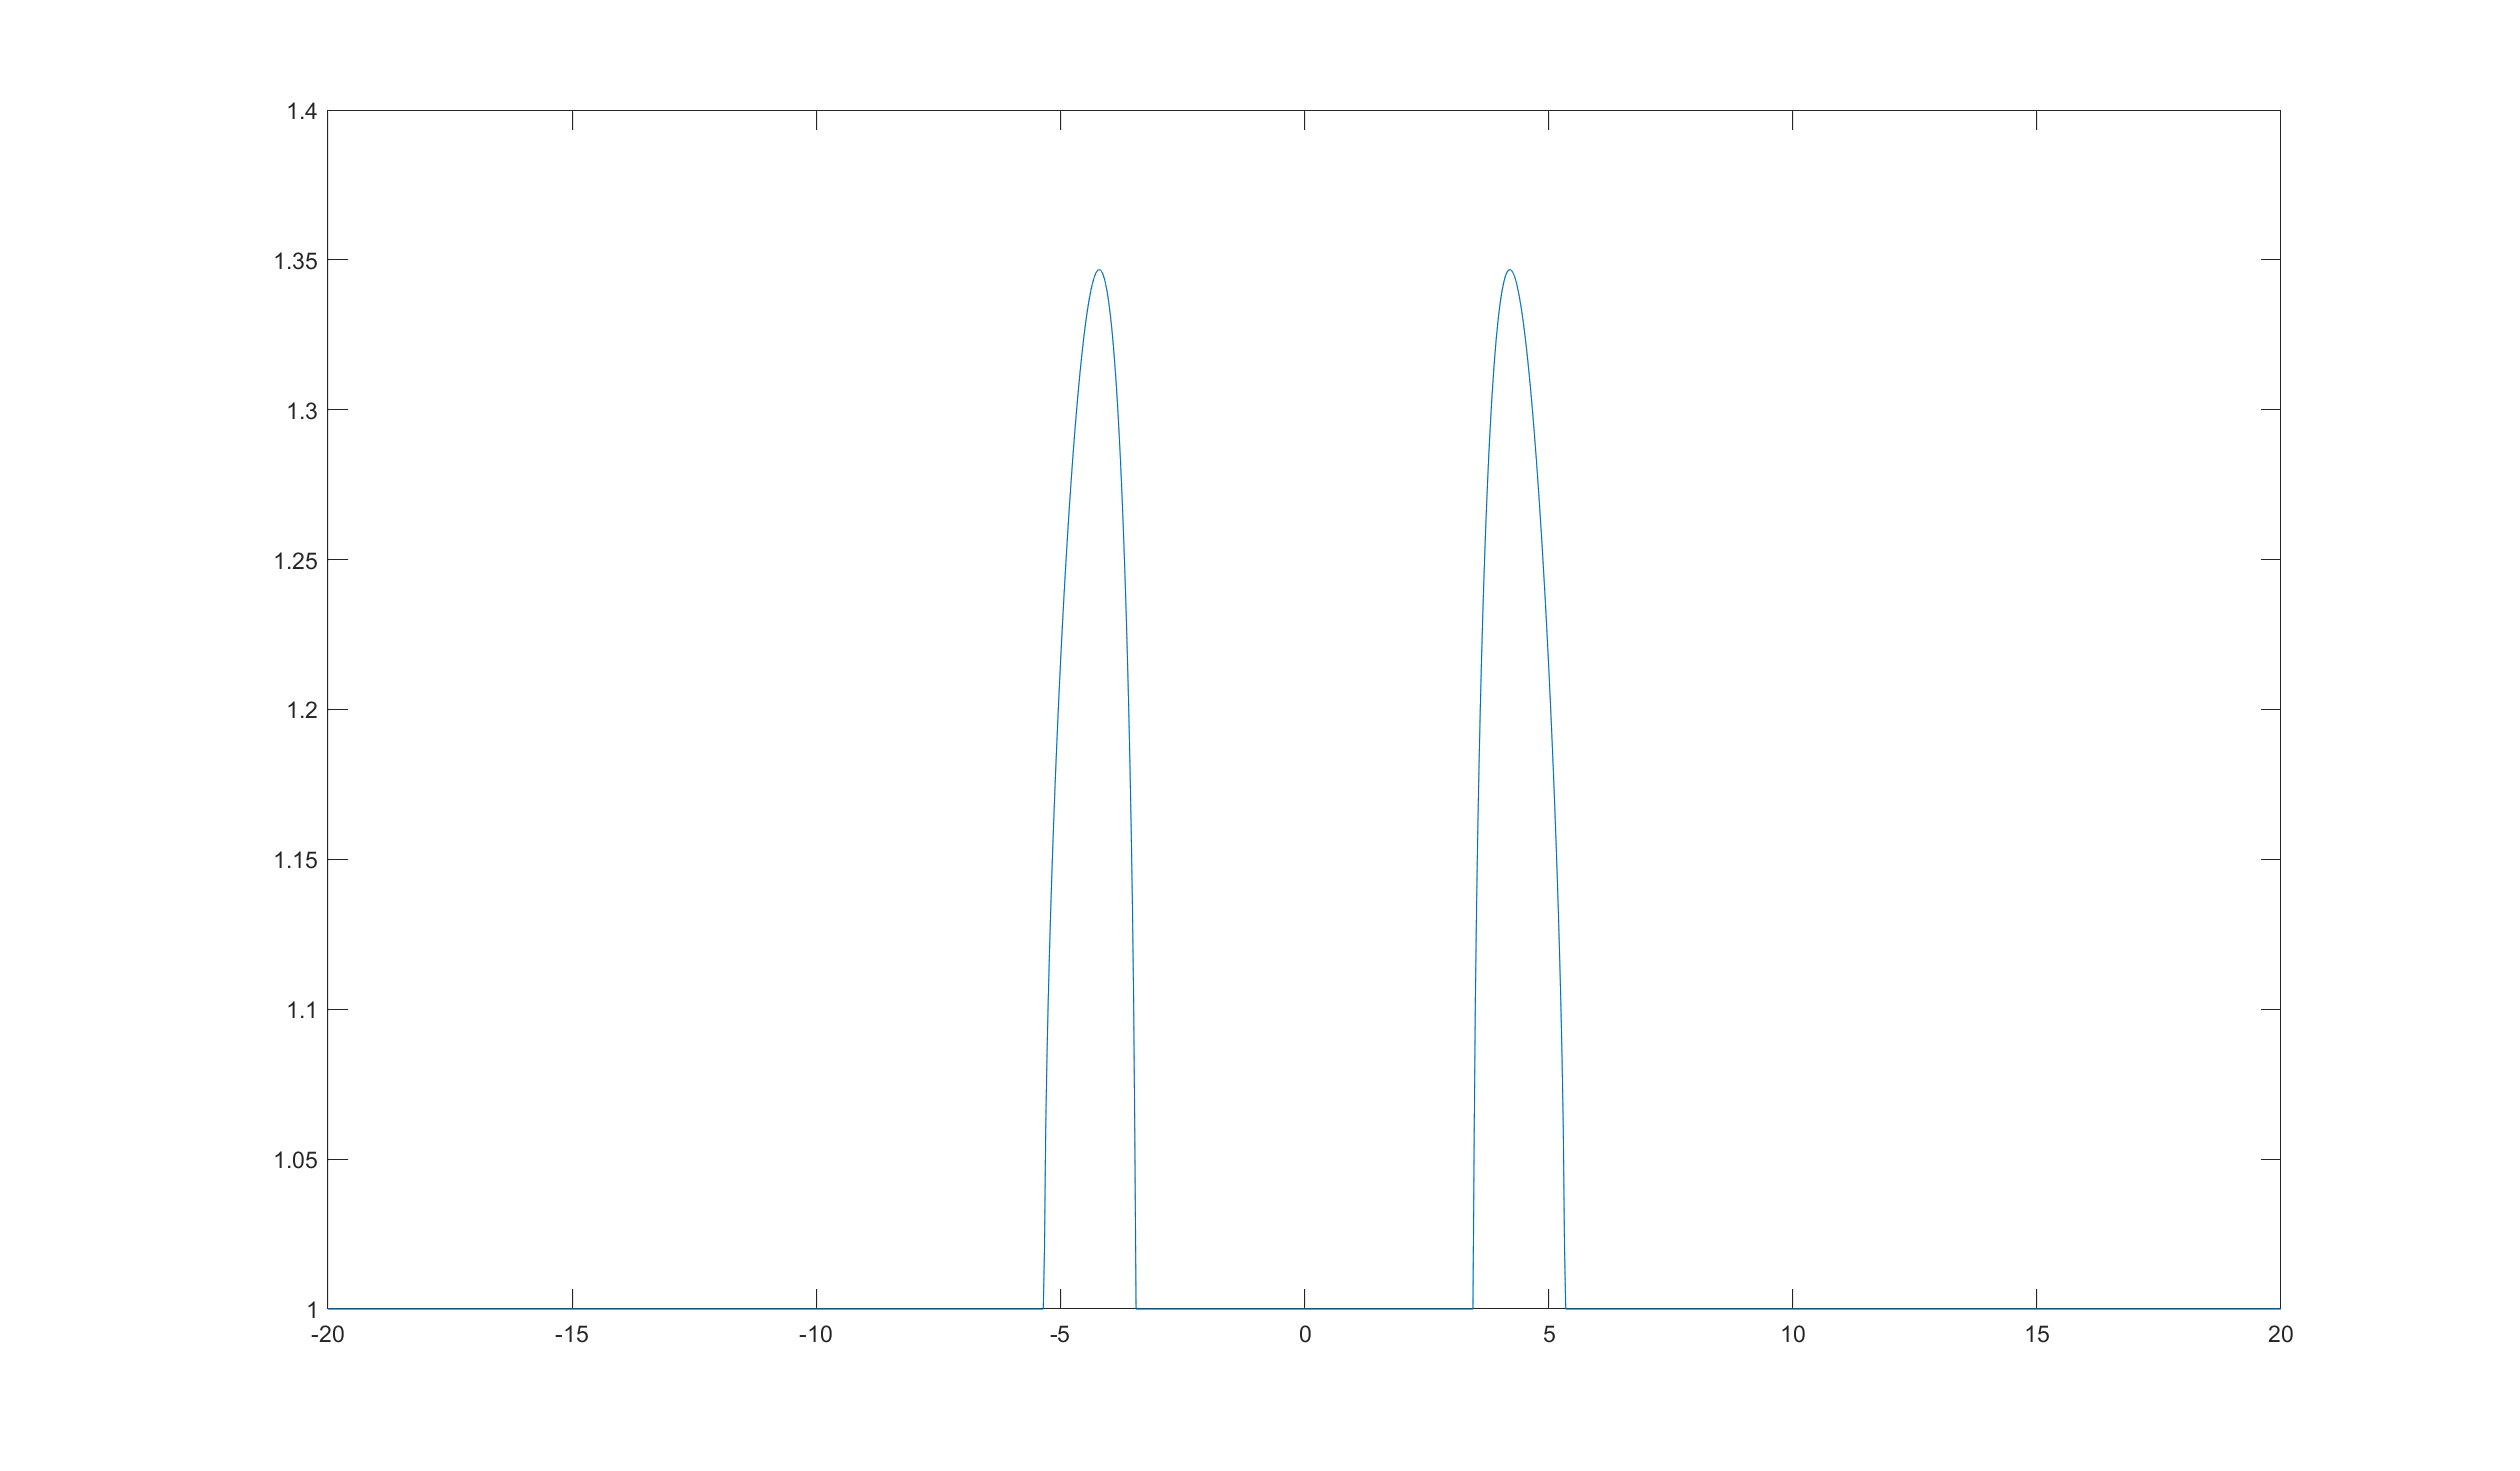
\includegraphics{images/2.jpg}
}
\caption{
\label{stab_area}
     M(z) при Re(z) = 0.}
\end{center}
\end{figure}
У функции есть небольшой всплеск от 3.45 до 5.35. Однако этот метод можно смело применять на практике. Как мы и убедились в \ref{numeric}. Считаю, что задачу 2 можно считать жетской.

Также был применен альтернативный подход из 2.2.2 \cite{stability}.
Были получены функции, представляющие собоб сумму по столбцам.
\begin{equation}
\begin{gathered}
R_{1} = \frac{(-11 + 6\sqrt{3})(13 z^{4} - 228\sqrt{3} z^{2} - 132 z^{2} - 576 \sqrt{3} - 432)}{13 (z^{4} - 12 \sqrt{3} z^{2} + 12 z^{2} + 288\sqrt{3} - 432)} + \\ \frac{12 (-5 + 3\sqrt{3}) (z^{2} + 6\sqrt{3} + 18) z}{z^{4} - 12\sqrt{3} z^{2} + 12 z^{2} + 288\sqrt{3} - 432}, \\
R_{2} = \frac{(-11 + 6\sqrt{3}) (13 z^{4} - 228\sqrt{3} z^{2} - 132 z^{2} - 576\sqrt{3} - 432)}{13 (z^{4} - 12\sqrt{3} z^{2} + 12 z^{2} + 288\sqrt{3} - 432)} + \\ \frac{(-2 + \sqrt{3}) (z^{2} + 12) (z^{2} - 12\sqrt{3}) z}{z^{4} - 12\sqrt{3} z^{2} + 12 z^{2} + 288\sqrt{3} - 432}
\end{gathered}
\end{equation}
Построим область $\lvert R_{1} \rvert \leq 1 \cap \lvert R_{2} \rvert \leq 1$.

\begin{figure}[ht]
\begin{center}
\scalebox{0.2}{
   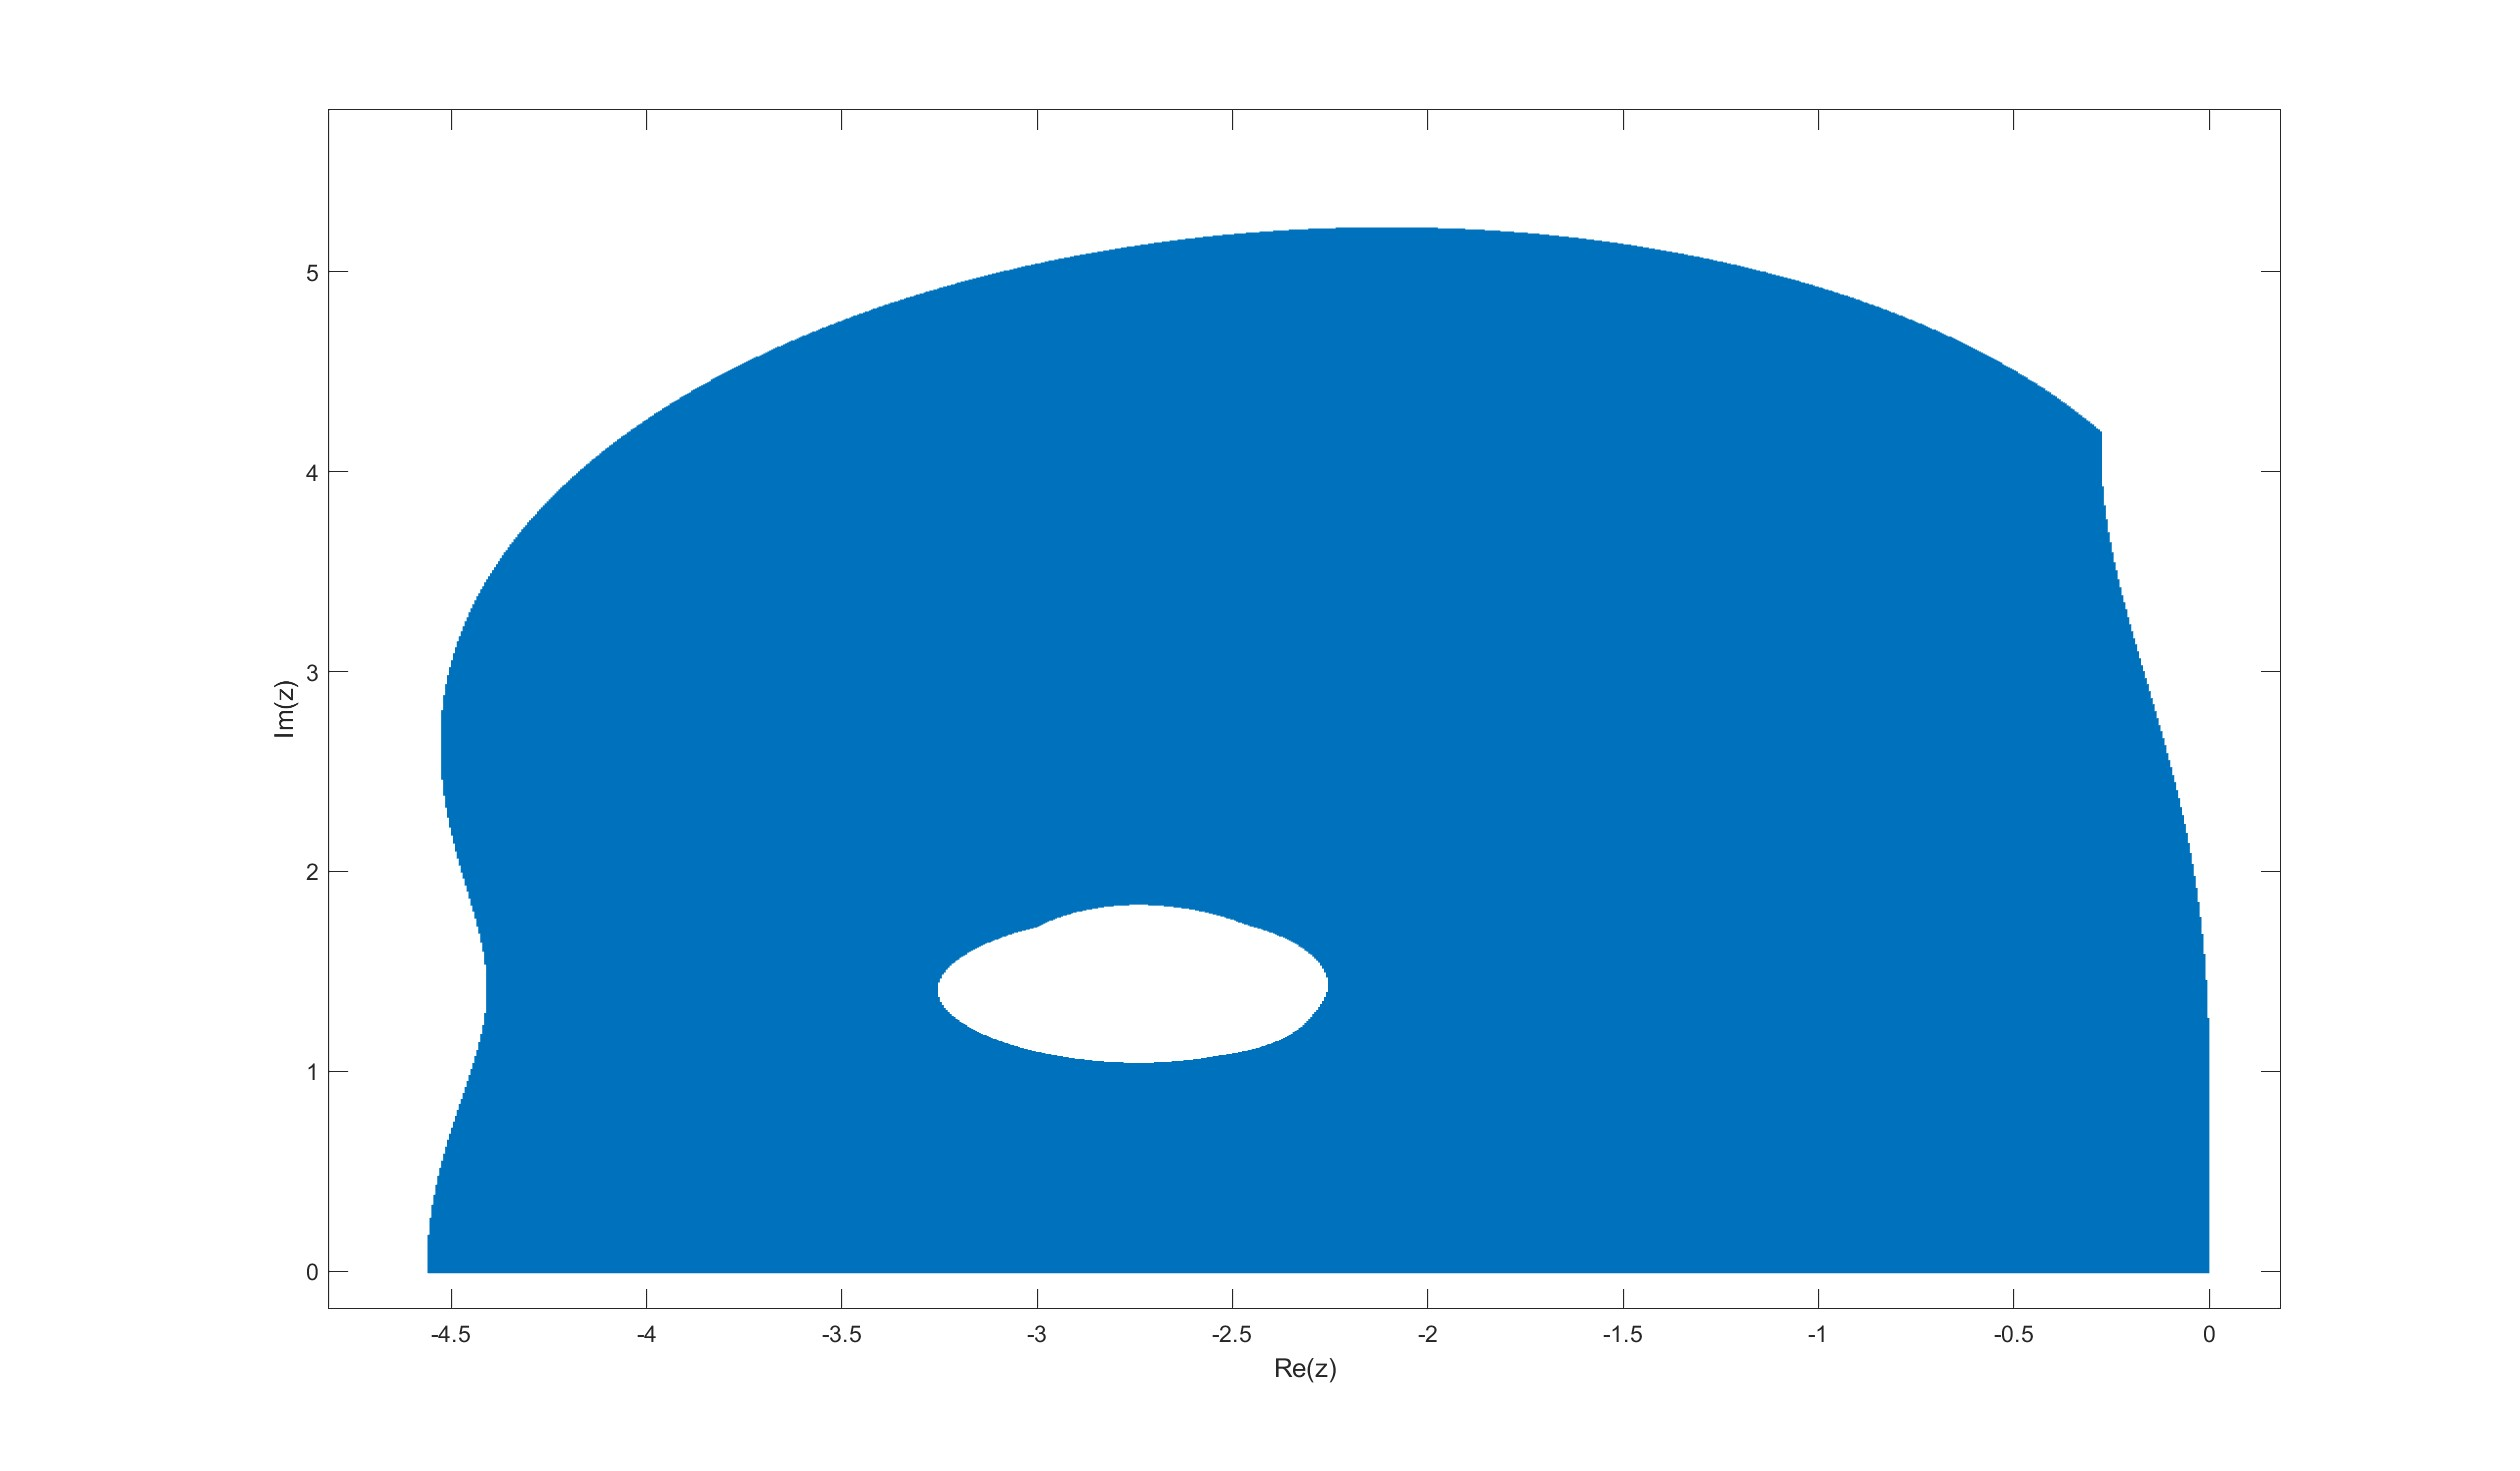
\includegraphics{images/1.jpg}
}
\caption{
\label{stab_area_another}
     $\lvert R_{1} \rvert \leq 1 \cap \lvert R_{2} \rvert \leq 1$}
\end{center}
\end{figure}

Область шире, чем у явного метода, однако не такая как у неявного. Из дальнейших рассуждений будет понятно, почему так происходит. 
\pagebreak

\begin{figure}[ht]
\begin{center}
\scalebox{0.5}{
   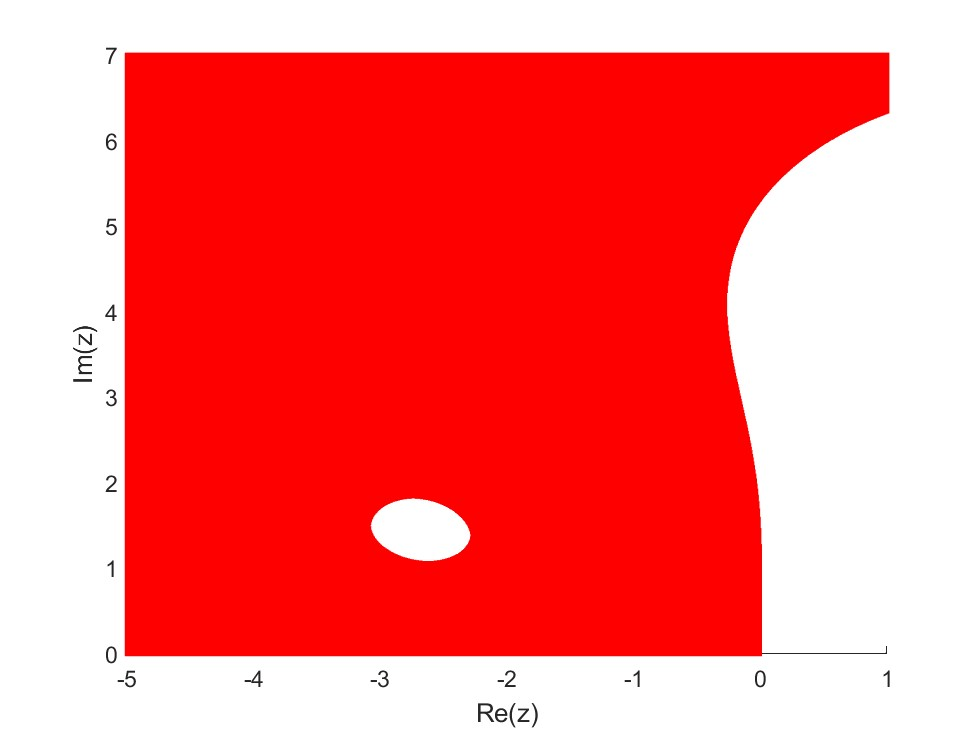
\includegraphics{images/4.jpg}
}
\caption{
\label{stab_area_another_1}
     $\lvert R_{1} \rvert \leq 1$}
\end{center}
\end{figure}

Данную область можно охарактеризовать как похожую на те, что принадлежат IRK. Из чего можем заключить, что область по первой компоненте неплохая.
\pagebreak

\begin{figure}[ht]
\begin{center}
\scalebox{0.5}{
   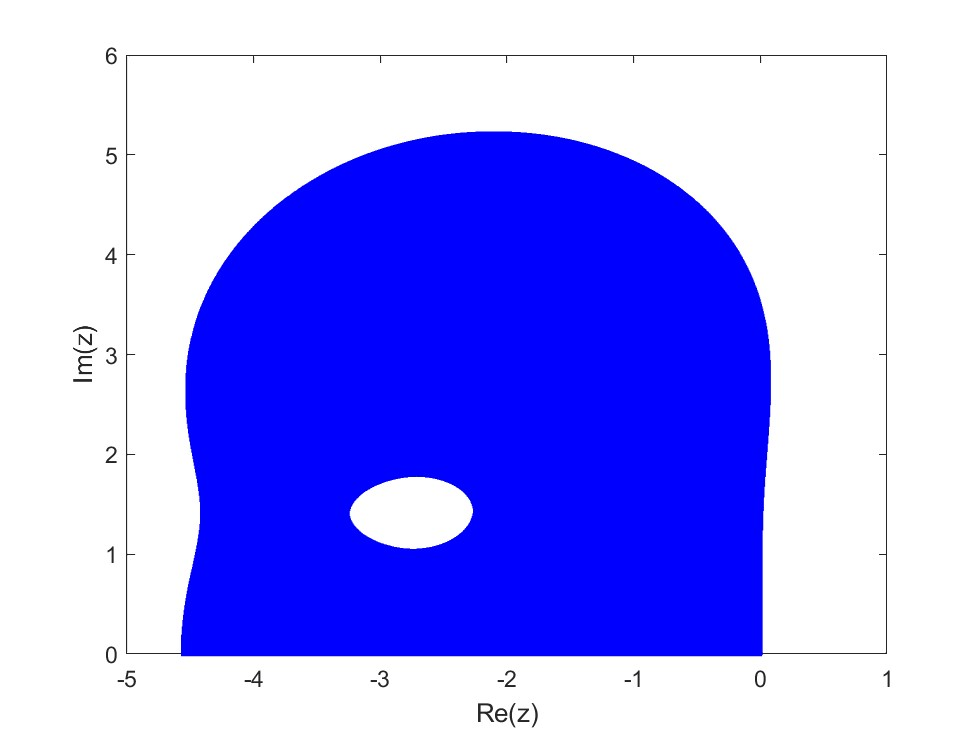
\includegraphics{images/5.jpg}
}
\caption{
\label{stab_area_another_2}
     $\lvert R_{2} \rvert \leq 1$}
\end{center}
\end{figure}

Однако тут результат достаточно плохой. По второй компоненте область похожа на область у классического РК, хотя и достаточно шире. Становится понятно, что из-за влияния второй компоненты пересечение похоже на явный метод.

Внутри области можно увидеть полую область, которая появляется из-за специфического вида функции устойчивости. А конкретно из-за того, что элементы представляют собой дроби.

Также стоит сказать, что возможно другие методы этого класса будет иметь лучшую область по сравнению с \ref{stab_area_another}.
\pagebreak

\specialsection{Выводы}

Был получен метод, который можно использовать на практике. Поскольку он требует меньшего количества вычислений чем IRK при достаточно хорошей точности. Однако в данной работе не был рассмотрен весь класс, а лишь предложен конкретный. Сформулирована схема для этого класса. Также были определены условия 4 порядка. При необходимости можно расширить рассуждения для большего порядка. В работе даны выкладки для нахождения функции устойчивости любого метода класса.
\pagebreak

\specialsection{Заключение}
По результатам работы был представлен целый класс методов. Представители должны хорошо работать на практике. Так как из-за его особенностей присутствую черты неявного метода. При этом решается задача для скалярного нелинейного вместо векторного нелинейного уравнения. Что сильно сказывается на вычислительной сложности.
\pagebreak

\begin{thebibliography}{1}
\bibitem{tree} Хайрер Э., Нёрсетт С., Ваннер Г. \flqq Решение обыкновенных дифференциальных уравнений\frqq~Издательство Москва Мир, 1990, C.~150--163.

\bibitem{Hofer1976} Hofer E. \flqq A partially implicit method for large stiff systems of ODEs with only few equations
introducing small time-constants\frqq~SIAM Journal Numerical Analytics, 1976, V.~13. I.~5. P.~645--663.

\bibitem{ShomeEtAl2004} Shome S. S., Haug E. J., Jay L. O. \flqq Dual-rate integration using partitioned Runge--Kutta methods for mechanical systems with interacting subsystems\frqq~Mechanics Based Design of Structures and Machines, 2004, V.~32. I.~3. P.~253--282.

\bibitem{SanduGuenther2016} Sandu A., Gunther M. \flqq Multirate generalized additive Runge--Kutta methods\frqq~Numerische Mathematik, 2016, V.~133. I.~3. P.~497--524.

\bibitem{KetchesonEtAl2016} Ketcheson D. I., MacDonald C., Ruuth S. J. \flqq Spatially partitioned embedded Runge--Kutta methods\frqq~SIAM Journal Numerical Analytics, 2013, V.~51. I.~5, P.~2887--2910

\bibitem{KalogiratouEtAl2011} Kalogiratou Z., Monovasilis T., Simos T. E. \flqq Symplectic partitioned Runge — Kutta methods for the numerical integration of periodic and oscillatory problems\frqq~Recent Advances in Computational and Applied Mathematics. Dordrecht, Springer Netherlands Publ., 2011, P.~169--208.

\bibitem{OlemskoyBook2009} Олемской И. В. \flqq Методы интегрирования систем структурно разделенных дифференциальных уравнений\frqq~СПб: Изд-во С.-Петерб. ун-та, 2009, C.~182

\bibitem{Olemskoy2003}  Олемской И. В. \flqq Структурный подход к задаче конструирования явных одношаговых методов\frqq~Ж. вычисл. матем. и матем. физ., 2003. Т.~43. №~7. C.~961--974.

\bibitem{Olemskoy2002} Олемской И. В. \flqq Четырехэтапный метод пятого порядка точности численного интегрирования систем специального вида\frqq~Ж. вычисл. матем. и матем. физ., 2002. Т.~42. №~8. C.~1179--1190.

\bibitem{Cash1975} Cash J. R. \flqq A class of implicit Runge-Kutta methods for the numerical integration of stiff differential systems\frqq~J. Assoc. Comput. Mach., 1975, V.~22. P.~504--511.

\bibitem{Bokhoven1980} Van Bokhoven W. M. G.\flqq Efficient higher order implicit one-step methods for integration of stiff differential equations\frqq~BIT, 1980, V.~20. P.~34--43.

\bibitem{Cash1982} Cash J. R. and Singhal A. \flqq Mono-implicit Runge-Kutta formulae for the numerical integration of stiff differential systems\frqq~IMA J. Numer. Anal., 1982, V.~2. P.~211--227.

\bibitem{Muir1987} Muir P. H. and Enright W. H. \flqq Relationships among some classes of IRK methods and their stability functions\frqq~BIT, 1987, V.~27. P.~403--423.

\bibitem{Cash1980} Cash J. R. and Moore D. R. \flqq A high order method for the numerical solution of two-point boundary value problems\frqq~BIT, 1980, V.~20. P.~44--52.

\bibitem{Enright1986} Enright W. H. and Muir P. H. \flqq Efficient classes of Runge-Kutta methods for two-point boundary value problems\frqq~Computing, 1986, V.~37. P.~315--334.

\bibitem{Gupta1985} Gupta S. \flqq An adaptive boundary value Runge-Kutta solver for first order boundary value prob-
lems\frqq~SIAM J. Numer. Anal., 1985, V.~22. P.~114--126.

\bibitem{Cash1991} Cash J. R. and Wright M. H. \flqq A deferred correction method for nonlinear two-point boundary
value problems: implementation and numerical evaluation\frqq~SIAM J. Sci. Statist. Comput., 1991, V.~12. P.~971--989.

\bibitem{Muir1993} Muir P. H. and Owren B. \flqq Order barriers and characterizations for continuous mono-implicit
Runge-Kutta schemes\frqq~Math. Comp., 1993, V.~61. N.~204. P.~675--699.

\bibitem{mirk} Burrage K., Chipman F. H., Muir P. H. \flqq Order results for Mono-Implicit Runge-Kutta methods\frqq~SIAM J. Numer. Anal., 1994, V.~31. N.~3. P.~876--891.

\bibitem{stability} Винничек Н. Н. \flqq Численная устойчивость разделяющихся методов решения систем обыкновенных дифференциальных уравнений.\frqq~Выпускная квалификационная работа магистра, Санкт-Петербургский государственный университет, фак-т ПМ-ПУ, 2018.

\bibitem{code} Программный код к настоящей ВКР [Электронный ресурс]. URL: https://github.com/potomushozhenya/qualifWork (Дата доступа: 19.05.2025).

\end{thebibliography}
\pagebreak

\specialsection{Приложение}
\end{document}